% lvlm_eval.tex — clean TikZ replacement for images/lvlm_eval.jpg
% Illustrates the three LVLM evaluation conditions on SOCO:
%   Vis.        — image query with REF keypoint
%   Vis+Desc.   — image query with REF keypoint  +  textual description
%   Desc.       — textual description only
% In every condition the LVLM must pick one of 4 candidates A/B/C/D on the target image.

\documentclass[border=4pt,tikz]{standalone}

\usepackage[T1]{fontenc}
\usepackage{lmodern}
\usepackage{xcolor}
\usepackage{tikz}
\usetikzlibrary{positioning,shapes.callouts,calc,fit,backgrounds}

% ---- palette (matches the SOCO project page) -------------------------------
\definecolor{socoBlue}{HTML}{2C69B0}
\definecolor{socoInk}{HTML}{1A2A3A}
\definecolor{socoGrid}{HTML}{D6DEE7}
\definecolor{socoMuted}{HTML}{5C6B7A}
\definecolor{refRed}{HTML}{E23A3A}
\definecolor{candGreen}{HTML}{2F8F4E}
\definecolor{carGrey}{HTML}{8A949E}

% ---- reusable styles --------------------------------------------------------
\tikzset{
  imgframe/.style={
    draw=socoInk, line width=0.6pt, rounded corners=1.5pt,
    fill=white
  },
  carbody/.style ={fill=socoBlue!75, draw=socoBlue!75},
  carcabin/.style={fill=socoBlue!85, draw=socoBlue!85},
  carwheel/.style={fill=socoInk, draw=socoInk},
  carwindow/.style={fill=socoBlue!20, draw=socoBlue!20},
  headcell/.style ={font=\sffamily\bfseries\small, text=socoInk},
  labelcell/.style={font=\sffamily\small,           text=socoInk},
}

% \carcard[<color>]{<center coord>}{<W>}{<H>}
% Side-view car schematic, front on the LEFT (long hood, slanted windshield).
% Optional first arg = base color; default socoBlue.
\newcommand{\carcard}[4][socoBlue]{%
  \begin{scope}[shift={#2}]
    \def\W{#3}\def\H{#4}
    \colorlet{cbody}{#1!75}
    \colorlet{ccabin}{#1!90}
    \colorlet{cwindow}{#1!22}
    \colorlet{chub}{#1!30}
    % frame
    \draw[imgframe] (-\W/2,-\H/2) rectangle (\W/2,\H/2);
    % ground line
    \draw[socoInk!25,line width=0.3pt]
      (-\W/2+\W*0.05,-\H*0.32) -- (\W/2-\W*0.05,-\H*0.32);
    % body (lower hull) — same rectangle, hood and rear differentiated by cabin shape
    \fill[cbody, rounded corners=1.2pt]
      (-\W*0.42,-\H*0.30) rectangle (\W*0.42,-\H*0.02);
    % small headlight at the front (left)
    \fill[yellow!85!orange]
      (-\W*0.40,-\H*0.10) rectangle (-\W*0.36,-\H*0.18);
    % cabin / roof — asymmetric: long slanted windshield on the front (left),
    % short steep rear glass on the right
    \fill[ccabin]
      (-\W*0.18,-\H*0.02) --   % windshield base (forward of center)
      ( \W*0.02, \H*0.22) --   % roof front
      ( \W*0.22, \H*0.22) --   % roof rear
      ( \W*0.30,-\H*0.02) --   % rear glass base
      cycle;
    % window strip (matches cabin shape, inset)
    \fill[cwindow]
      (-\W*0.13,-\H*0.02 + \H*0.02) --
      ( \W*0.04, \H*0.18) --
      ( \W*0.20, \H*0.18) --
      ( \W*0.26,-\H*0.02 + \H*0.02) --
      cycle;
    % subtle window mullion between front and rear glass
    \draw[cbody,line width=0.5pt]
      ( \W*0.12, \H*0.18) -- ( \W*0.12,-\H*0.02 + \H*0.02);
    % wheels — front-left (under windshield base) and rear (under rear-glass)
    \fill[carwheel] (-\W*0.22,-\H*0.30) circle (\W*0.08);
    \fill[carwheel] ( \W*0.26,-\H*0.30) circle (\W*0.08);
    % wheel hubs
    \fill[chub] (-\W*0.22,-\H*0.30) circle (\W*0.030);
    \fill[chub] ( \W*0.26,-\H*0.30) circle (\W*0.030);
  \end{scope}
}

% red REF dot at given offset relative to card center
% \refdot{<card center>}{<dx>}{<dy>}
\newcommand{\refdot}[3]{%
  \begin{scope}[shift={#1}]
    \draw[fill=refRed,draw=white,line width=0.4pt] (#2,#3) circle (0.085);
  \end{scope}
}

% target candidates on a car card
% \candidates{<card center>}{<W>}{<H>}
\newcommand{\candidates}[3]{%
  \begin{scope}[shift={#1}]
    \def\W{#2}\def\H{#3}
    % positions relative to card center, chosen to sit on distinct car parts:
    %   A — front-left wheel (correct answer)
    %   B — rear-right wheel
    %   C — front bumper / headlight
    %   D — roof corner (rear)
    % label offset (lx,ly) keeps the letter clear of the dot and the car body.
    \foreach \name/\x/\y/\lx/\ly in {%
        A/-0.22/-0.30/-0.28/-0.50,%
        B/ 0.26/-0.30/ 0.32/-0.50,%
        C/-0.40/-0.14/-0.48/-0.16,%
        D/ 0.22/ 0.22/ 0.30/ 0.34}{%
      \draw[fill=candGreen,draw=white,line width=0.3pt]
        (\x*\W,\y*\H) circle (0.06);
      \node[font=\sffamily\scriptsize\bfseries,text=candGreen]
        at (\lx*\W,\ly*\H) {\name};
    }
  \end{scope}
}

% =============================================================================
\begin{document}
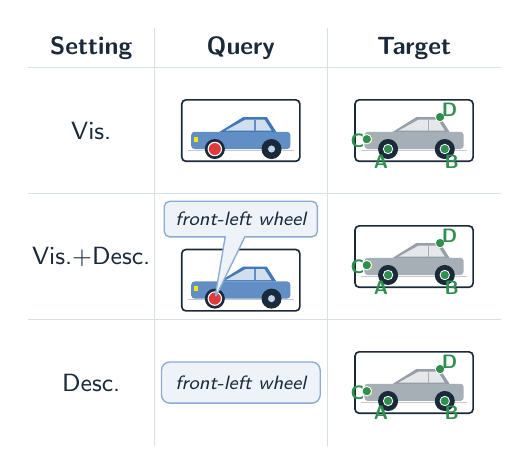
\begin{tikzpicture}[
  x=1cm,y=1cm,
  every node/.style={inner sep=0pt,outer sep=0pt},
]

% --- geometry ---------------------------------------------------------------
\def\colA{1.6}     % "Setting" column width
\def\colB{2.2}     % "Query" column width (just wide enough for the card)
\def\colC{2.2}     % "Target" column width
\def\rowH{1.6}     % body row height (tighter)
\def\headH{0.5}    % header row height

\def\imgW{1.50}    % card width
\def\imgH{0.78}    % card height

\def\imgYshift{-0.30}  % how far below row centre the image sits in rows 2/3
\def\bubYshift{ 0.25}  % how far above row centre the bubble sits in row 2

% column x-centers
\pgfmathsetmacro{\xA}{\colA/2}
\pgfmathsetmacro{\xB}{\colA + \colB/2}
\pgfmathsetmacro{\xC}{\colA + \colB + \colC/2}
\pgfmathsetmacro{\xTot}{\colA + \colB + \colC}

% row y-centers (top → bottom)
\pgfmathsetmacro{\ryh}{0}
\pgfmathsetmacro{\rya}{-\headH/2 - \rowH/2}
\pgfmathsetmacro{\ryb}{\rya - \rowH}
\pgfmathsetmacro{\ryc}{\ryb - \rowH}

\pgfmathsetmacro{\rytop}{\headH/2}
\pgfmathsetmacro{\rybot}{-\headH/2 - 3*\rowH}

% --- background separators --------------------------------------------------
\begin{scope}[on background layer]
  \draw[socoGrid,line width=0.4pt] (0,-\headH/2) -- (\xTot,-\headH/2);
  \draw[socoGrid,line width=0.4pt] (0,\rya-\rowH/2) -- (\xTot,\rya-\rowH/2);
  \draw[socoGrid,line width=0.4pt] (0,\ryb-\rowH/2) -- (\xTot,\ryb-\rowH/2);
  \draw[socoGrid,line width=0.4pt] (\colA,\rytop) -- (\colA,\rybot);
  \draw[socoGrid,line width=0.4pt] (\colA+\colB,\rytop) -- (\colA+\colB,\rybot);
\end{scope}

% --- header row -------------------------------------------------------------
\node[headcell] at (\xA,\ryh) {Setting};
\node[headcell] at (\xB,\ryh) {Query};
\node[headcell] at (\xC,\ryh) {Target};

% REF dot offsets — front-left wheel of the car (matches \candidates A position)
\pgfmathsetmacro{\refDX}{-0.22*\imgW}
\pgfmathsetmacro{\refDY}{-0.30*\imgH}

% --- Row 1: Vis. ------------------------------------------------------------
\node[labelcell] at (\xA,\rya) {Vis.};
\carcard{(\xB,\rya)}{\imgW}{\imgH}
\refdot{(\xB,\rya)}{\refDX}{\refDY}

% --- Row 2: Vis + Desc. -----------------------------------------------------
\node[labelcell,align=center] at (\xA,\ryb) {Vis.+Desc.};
% image sits in lower half of the row, bubble above
\pgfmathsetmacro{\yBimg}{\ryb + \imgYshift}
\pgfmathsetmacro{\yBbub}{\ryb + \bubYshift}
\carcard{(\xB,\yBimg)}{\imgW}{\imgH}
\refdot{(\xB,\yBimg)}{\refDX}{\refDY}
% bubble centred above the image, pointer down at the REF dot
\coordinate (refdot2) at ($(\xB,\yBimg)+(\refDX,\refDY)$);
\node[
  rectangle callout, rounded corners=2pt,
  callout absolute pointer={(refdot2)},
  draw=socoBlue!55, line width=0.5pt, fill=socoBlue!8,
  inner sep=4pt, font=\sffamily\scriptsize\itshape,
  text=socoInk, align=center,
  anchor=south
] at (\xB,\yBbub) {front-left wheel};

% --- Row 3: Desc. -----------------------------------------------------------
\node[labelcell] at (\xA,\ryc) {Desc.};
% standalone bubble, centred — plain rounded rectangle (no pointer)
\node[
  rectangle, rounded corners=3pt,
  draw=socoBlue!55, line width=0.5pt, fill=socoBlue!8,
  inner sep=5pt, font=\sffamily\scriptsize\itshape,
  text=socoInk, align=center
] at (\xB,\ryc) {front-left wheel};

% --- Target column: same target car in all three rows, grey to distinguish --
\foreach \yy in {\rya,\ryb,\ryc}{
  \carcard[carGrey]{(\xC,\yy)}{\imgW}{\imgH}
  \candidates{(\xC,\yy)}{\imgW}{\imgH}
}

\end{tikzpicture}
\end{document}
